\documentclass[german]{../spicker}

\usepackage{amsmath}

\usepackage{graphicx}
\usepackage{tabularx, multirow}

\usetikzlibrary{arrows.meta,chains,decorations.pathreplacing,scopes,shapes.misc}

\addbibresource{algo.bib}

\title{Algorithmen}
\author{Patrick Gustav Blaneck}
\makeindex[intoc]
\makeindex[intoc, name=Beispiele,title=Beispiele]

\newenvironment{allintypewriter}{\ttfamily}{\par}

 
\pgfmathsetmacro\twopi{2*pi}

\pgfmathdeclarefunction{lngamma}{1}{%
  \pgfmathsetmacro\lngammatmp{#1*#1*#1}%
  \pgfmathparse{%
    #1*ln(#1) - #1 - .5*ln(#1/\twopi)
    + 1/12/#1 - 1/360/\lngammatmp + 1/1260/\lngammatmp/#1/#1
  }%
}  

\pgfmathdeclarefunction{facreal}{1}{%
  \pgfmathparse{exp(lngamma(#1+1))}% 
}

\begin{document}
\maketitle
\tableofcontents
\newpage

%\setcounter{section}{1}

\section{Grundbegriffe}
\begin{defi}{Eigenschaften eines Algorithmus}
    \begin{itemize}
        \item \emph{Terminierung:} Der Algorithmus bricht nach \emph{endlichen vielen} Schritten ab.
        \item \emph{Determiniertheit:} Bei vorgegebener Eingabe wird ein eindeutiges \emph{Ergebnis} geliefert.
        \item \emph{Determinismus:} Eindeutige Vorgabe der \emph{Abfolge} der auszuführenden Schritte
    \end{itemize}
\end{defi}

\subsection{Algorithmische Komplexität}

\begin{defi}{Landau-Notation}
    Seien $f, g$ reellwertige Funktionen der reellen Zahlen.
    Dann gilt: \cite{wiki:Landau-Symbole}

    \begin{tabular}{l|l|l}
        Notation          & Definition       & Mathematische Definition                                                                                                  \\
        \hline
        $f \in \bigo(g)$  & obere Schranke   & $\exists C > 0 \exists x_0 > 0 \forall x > x_0 : \abs{f(x)} \leq C \cdot \abs{g(x)}$                                      \\
        $f \in \Omega(g)$ & untere Schranke  & $\exists c > 0 \exists x_0 > 0 \forall x > x_0 : c\cdot \abs{g(x)} \leq \abs{f(x)}$                                       \\
        $f \in \Theta(g)$ & scharfe Schranke & $\exists c > 0 \exists C > 0 \exists x_0 > 0 \forall x > x_0 : c\cdot \abs{g(x)} \leq \abs{f(x)} \leq C \cdot \abs{g(x)}$ \\
    \end{tabular}

    Anschaulicher gilt:

    \begin{tabular}{l|l}
        Notation          & Anschauliche Bedeutung                        \\
        \hline
        $f \in \bigo(g)$  & $f$ wächst nicht wesentlich schneller als $g$ \\
        $f \in \Omega(g)$ & $f$ wächst nicht wesentlich langsamer als $g$ \\
        $f \in \Theta(g)$ & $f$ wächst genauso schnell wie $g$
    \end{tabular}
\end{defi}

\begin{example}{Landau-Notation}
    Aus \cite{wiki:Landau-Symbole} :

    \begin{tabular}{l|l}
        Notation                & Beispiel                                          \\
        \hline
        $f \in \bigo(1)$        & Feststellen, ob eine Binärzahl gerade ist         \\
        $f \in \bigo(\log n)$   & Binäre Suche im sortierten Feld mit $n$ Einträgen \\
        $f \in \bigo(\sqrt{n})$ & Anzahl der Divisionen des naiven Primzahltests    \\
        $f \in \bigo(n)$        & Suche im unsortierten Feld mit $n$ Einträgen      \\
        $f \in \bigo(n\log n)$  & Mergesort, Heapsort                               \\
        $f \in \bigo(n^2)$      & Selectionsort                                     \\
        $f \in \bigo(n^m)$      &                                                   \\
        $f \in \bigo(2^{cn})$   & (Backtracking)                                    \\
        $f \in \bigo(n!)$       & Traveling Salesman Problem
    \end{tabular}
\end{example}

\begin{bonus}{Visualisierung Komplexitätsklassen}
    \begin{center}
        \begin{tikzpicture}[scale=1]
            \begin{axis}[
                    %view={45}{15},
                    width=15cm,
                    unit vector ratio*=1 1,
                    axis lines = middle,
                    grid=major,
                    ymin=0,
                    ymax=50,
                    xmin=0,
                    xmax=50,
                    %zmin=-1,
                    %zmax=10,
                    xlabel = $n$,
                    ylabel = $N$,
                    %zlabel = $z$,
                    %xtick style={draw=none},
                    %ytick style={draw=none},
                    %ztick style={draw=none},
                    xtick distance={5},
                    ytick distance={5},
                    %ztick distance={1},
                    %xticklabels=\empty,
                    %yticklabels=\empty,
                    %zticklabels=\empty,
                    disabledatascaling,
                    %stack dir=minus,
                    cycle list name=color list,
                    samples=250,
                    solid,
                    smooth,
                    line width=1.0pt,
                    no markers,
                    legend cell align={left},
                    reverse legend,
                ]

                \addplot +[domain=0:50]{0};         \addlegendentry{$\bigo(1)$};
                \addplot +[domain=0:50]{ln(x)};     \addlegendentry{$\bigo(\log(n))$};
                \addplot +[domain=0:50]{sqrt(x)};   \addlegendentry{$\bigo(\sqrt{n})$};
                \addplot +[domain=0:50]{x};         \addlegendentry{$\bigo(n)$};
                \addplot +[domain=0:50]{x * ln(x)}; \addlegendentry{$\bigo(n \log(n))$};
                \addplot +[domain=0:50]{x^2};       \addlegendentry{$\bigo(n^2)$};
                \addplot +[domain=0:10]{2^x};        \addlegendentry{$\bigo(2^n)$};
                \addplot +[domain=0:5]{facreal(x)}; \addlegendentry{$\bigo(n!)$};
            \end{axis}
        \end{tikzpicture}
    \end{center}
\end{bonus}

\newpage
\section{Elementare Datenstrukturen}

\begin{defi}{Homogene Datenstruktur}
    In einer \emph{homogenen Datenstruktur} haben alle Komponenten den \emph{gleichen} Datentyp.
\end{defi}

\begin{defi}{Heterogene Datenstruktur}
    In einer \emph{heterogenen Datenstruktur} haben die Komponenten \emph{unterschiedliche} Datentypen.
\end{defi}

% ADTs
\begin{defi}{Abstrakte Datentupen (ADTs)}
    Anforderungen an die Definition eines Datentyps:
    \begin{itemize}
        \item \emph{Spezifikation} eines Datentyps unabhängig von der Implementierung
        \item Reduzierung der von außen sichtbaren Aspekte auf die \emph{Schnittstelle} des Datentyps
    \end{itemize}

    Daraus entstehen \textbf{zwei Prinzipien}:
    \begin{itemize}
        \item \emph{Kapselung:}
              \subitem Zu einem ADT gehört eine Schnittstelle.
              \subitem Zugriffe auf den ADT erfolgen ausschließlich über die Schnittstelle.
        \item \emph{Geheimnisprinzip:}
              \subitem Interne Realisierung eines ADT-Moduls bleibt verborgen.
    \end{itemize}
\end{defi}

\begin{example}{ADT in Java}
    Viele wichtige abstrakte Datentypen werden in Java durch \emph{Interfaces} beschrieben.

    Es gibt ein oder mehrere Implementierungen dieser Interfaces mit unterschiedlichen dahinter stehenden Konzepten.

    In Java: Package \texttt{java.util}

    Wichtig in der Vorlesung:

    \begin{tabular}{l|l|l}
        ADT                     & Grund-ADT/Interface & Java-Klassen                      \\
        \hline
        Feld                    &                     & (Felder), HashMap                 \\
        Liste                   & List                & ArrayList, LinkedList             \\
        Menge                   & Set                 & HashSet, TreeSet                  \\
        Prioritätswarteschlange &                     & PriorityQueue                     \\
        Stack                   & List                &                                   \\
        Queue                   & List                &                                   \\
        Deque                   & List                & Deque (Interface), ArrayDeque     \\
        Map                     & Set                 & Map (Interface), HashMap, TreeMap \\
        BidiMap                 & Map                 & BidiMap, BiMap (Interface)        \\
        MultiSet, Bag           & Map                 & Bag, Multiset (Interface)
    \end{tabular}
\end{example}

\subsection{Felder und abstrakte Datenstrukturen}

\begin{defi}{Array}
    Ein \emph{Array} hat folgende spezielle Eigenschaften:
    \begin{itemize}
        \item Feste Anzahl an Datenobjekten
        \item Auf jedes Objekt kann direkt lesend oder schreibend zugegriffen werden
    \end{itemize}

    \begin{center}
        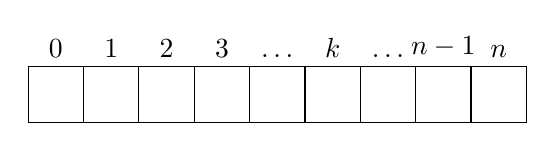
\begin{tikzpicture}[
                %  -{Stealth[length = 2.5pt]},
                start chain,
                node distance = 0pt,
                StackBlock/.style={draw, minimum width=2em, minimum height=2em, outer sep=0pt, on chain},
            ]
            { start chain = going right
                \node [StackBlock, label=$0$] (0) {};
                \node [StackBlock, label=$1$] (1) {};
                \node [StackBlock, label=$2$] (2) {};
                \node [StackBlock, label=$3$] (3) {};
                \node [StackBlock, label=$\ldots$] (d1) {};
                \node [StackBlock, label=$k$] (k) {};
                \node [StackBlock, label=$\ldots$] (d2) {};
                \node [StackBlock, label=$n-1$] (n1) {};
                \node [StackBlock, label=$n$] (n) {};
            }
        \end{tikzpicture}
    \end{center}

    \textbf{Performance:}

    \begin{center}
        \begin{tabular}{c|c|c|c|c}
            Zugriff     & Suche       & Einf./Lösch. (Anfang) & Einf./Lösch. (Ende) & Einf./Lösch. (Mitte) \\
            \hline
            $\Theta(1)$ & $\Theta(n)$ & -                     & -                   & -                    \\
        \end{tabular}
    \end{center}
\end{defi}

% Listen
\begin{defi}{Liste (Einfach verkettete)}
    Für eine \emph{Liste} kommt im Vergleich zu einem Array hinzu:
    \begin{itemize}
        \item Eine Liste kann wachsen und schrumpfen.
    \end{itemize}

    \begin{center}
        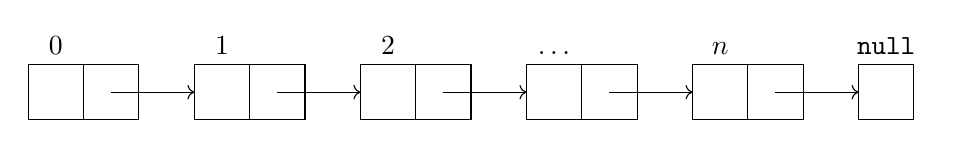
\begin{tikzpicture}[
                %  -{Stealth[length = 2.5pt]},
                start chain,
                node distance = 0pt,
                StackBlock/.style={draw, minimum width=2em, minimum height=2em, outer sep=0pt, on chain},
            ]
            { start chain = going right
                \node [StackBlock, label=$0$] (0) {};
                \node [StackBlock] (0p) {};
                \node [StackBlock, label=$1$,xshift=2em] (1) {};
                \node [StackBlock] (1p) {};
                \node [StackBlock, label=$2$,xshift=2em] (2) {};
                \node [StackBlock] (2p) {};
                \node [StackBlock, label=$\ldots$,xshift=2em] (dots) {};
                \node [StackBlock] (dotsp) {};
                \node [StackBlock, label=$n$,xshift=2em] (n) {};
                \node [StackBlock] (np) {};
                \node [StackBlock, label=\texttt{null}, xshift=2em] (null) {};


                \draw[->] (0p.center) [out=0, in=180] to (1.west);
                \draw[->] (1p.center) [out=0, in=180] to (2.west);
                \draw[->] (2p.center) [out=0, in=180] to (dots.west);
                \draw[->] (dotsp.center) [out=0, in=180] to (n.west);
                \draw[->] (np.center) [out=0, in=180] to (null.west);
            }
        \end{tikzpicture}
    \end{center}

    \textbf{Performance:}

    \begin{center}
        \begin{tabular}{c|c|c|c|c}
            Zugriff     & Suche       & Einf./Lösch. (Anfang) & Einf./Lösch. (Ende)                                                                                 & Einf./Lösch. (Mitte)   \\
            \hline
            $\Theta(n)$ & $\Theta(n)$ & $\Theta(1)$           & $\Theta(1)/\Theta(n)$\footnote{$\Theta(1)$, wenn das letzte Element bekannt ist, $\Theta(n)$ sonst} & Suchzeit + $\Theta(1)$ \\
        \end{tabular}
    \end{center}
\end{defi}

% Dynamische Felder
\begin{defi}{Dynamisches Feld}
    Ein \emph{dynamisches Feld} besteht aus:
    \begin{itemize}
        \item Einem normalen Feld, das nicht vollständig gefüllt ist.
        \item Einem Zeiger, der anzeigt, welches das erste unbesetzte Element ist.
    \end{itemize}

    \begin{center}
        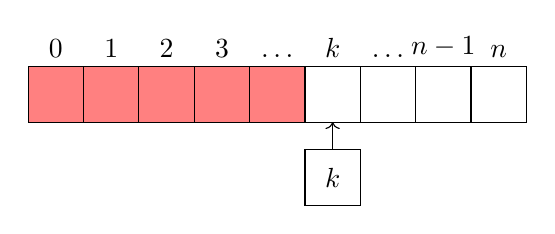
\begin{tikzpicture}[
            %  -{Stealth[length = 2.5pt]},
            start chain,
            node distance = 0pt,
            StackBlock/.style={draw, minimum width=2em, minimum height=2em, outer sep=0pt, on chain},
            ]
            { start chain = going right
            \node [StackBlock, fill=red!50, label=$0$] (0) {};
            \node [StackBlock, fill=red!50, label=$1$] (1) {};
            \node [StackBlock, fill=red!50, label=$2$] (2) {};
            \node [StackBlock, fill=red!50, label=$3$] (3) {};
            \node [StackBlock, fill=red!50, label=$\ldots$] (d1) {};
            \node [StackBlock, label=$k$] (k) {};
            \node [StackBlock, label=$\ldots$] (d2) {};
            \node [StackBlock, label=$n-1$] (n1) {};
            \node [StackBlock, label=$n$] (n) {};

            { [continue chain = going below]
            \chainin (k);
            \node[StackBlock,yshift=-1em] (pointer) {$k$};
            \draw[->] (pointer.north) [out=90, in=-90] to (k.south);
            }

            }
            %\begin{scope}[-{Stealth[length = 2.5pt]}]
            %\draw (1.north) [out=25, in=155] to (2.north);
            %\draw (1.north) [out=30, in=155] to (3.north);
            %\draw (1.north) [out=35, in=155] to (4.north);
            %\draw (6.north) [out=40, in=155] to (6.north);
            %\end{scope}
            %\draw[decorate,decoration={brace, amplitude=10pt, raise=5pt, mirror}]
            %(2.south west) to node[black,midway,below= 15pt] {$k$-elements} (7.south east);%

        \end{tikzpicture}
    \end{center}

    \textbf{Performance:}

    \begin{center}
        \begin{tabular}{c|c|c|c|c}
            Zugriff     & Suche       & Einf./Lösch. (Anfang) & Einf./Lösch. (Ende)                                                                                     & Einf./Lösch. (Mitte) \\
            \hline
            $\Theta(1)$ & $\Theta(n)$ & $\Theta(n)$           & $\Theta(1)/\Theta(n)$\footnote{Wenn das Feld schon voll ist, muss der komplette Inhalt kopiert werden.} & $\Theta(n)$          \\
        \end{tabular}
    \end{center}

    \textbf{Implementierung:}
    \begin{itemize}
        \item Ein dynamisches Feld ist für einen Stack gut geeignet:
              \subitem Einfügen am Ende: $\Theta(1)$ (aber: Worst-Case $\Theta(n)$!)
              \subitem Auslesen am Ende: $\Theta(1)$
    \end{itemize}
\end{defi}

% Zirkuläre dynamische Felder
\begin{defi}{Zirkuläres (dynamisches) Feld}
    Ein \emph{zirkuläres Feld} besitzt einen Speicher fester Größe.
    Dabei speichern zwei Zeiger jeweils den Anfang (\texttt{head}) des Speichers, bzw. auf die nächste freie Speicheradresse (\texttt{tail}) im Speicher.

    Wird ein Element am Anfang \glqq abgearbeitet\grqq, bewegt sich \texttt{head} eine Position weiter.
    Wird ein Element am Ende eingefügt, bewegt sich \texttt{tail} eine Position weiter.
    \begin{center}
        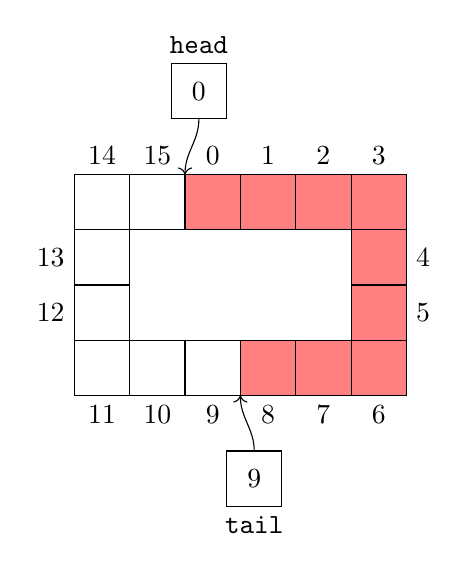
\begin{tikzpicture}[
            %  -{Stealth[length = 2.5pt]},
            start chain,
            node distance = 0pt,
            StackBlock/.style={draw, minimum width=2em, minimum height=2em, outer sep=0pt, on chain},
            ]
            { start chain = going right
            \node [StackBlock,label=above:$15$] (15) {};
            \node [StackBlock,label=above:$0$, fill=red!50] (0) {};
            \node [StackBlock,label=above:$1$, fill=red!50] (1) {};
            \node [StackBlock,label=above:$2$, fill=red!50] (2) {};
            \node [StackBlock,label=above:$3$, fill=red!50] (3) {};

            { [continue chain = going below]
            \chainin (3);
            \node [StackBlock,label=right:$4$, fill=red!50] (4) {};
            \node [StackBlock,label=right:$5$, fill=red!50] (5) {};
            \node [StackBlock,label=below:$6$, fill=red!50] (6) {};
            }

            { [continue chain = going left]
            \chainin (6);
            \node [StackBlock,label=below:$7$, fill=red!50] (7) {};
            \node [StackBlock,label=below:$8$, fill=red!50] (8) {};
            \node [StackBlock,label=below:$9$] (9) {};
            \node [StackBlock,label=below:$10$] (10) {};
            \node [StackBlock,label=below:$11$] (11) {};
            }

            { [continue chain = going above]
            \chainin (11);
            \node [StackBlock,label=left:$12$] (12) {};
            \node [StackBlock,label=left:$13$] (13) {};
            \node [StackBlock,label=above:$14$] (14) {};
            }


            { [continue chain = going above]
            \chainin (0);
            \node[StackBlock,yshift=2em,xshift=-0.5em,label=\texttt{head}] (head) {$0$};
            \draw[->] (head.south) [out=-90, in=90] to (0.north west);
            }

            { [continue chain = going below]
            \chainin (9);
            \node[StackBlock,yshift=-2em,xshift=1.5em,label=below:\texttt{tail}] (tail) {$9$};
            \draw[->] (tail.north) [out=90, in=-90] to (9.south east);
            }
            }
            %\begin{scope}[-{Stealth[length = 2.5pt]}]
            %\draw (1.north) [out=25, in=155] to (2.north);
            %\draw (1.north) [out=30, in=155] to (3.north);
            %\draw (1.north) [out=35, in=155] to (4.north);
            %\draw (6.north) [out=40, in=155] to (6.north);
            %\end{scope}
            %\draw[decorate,decoration={brace, amplitude=10pt, raise=5pt, mirror}]
            %(2.south west) to node[black,midway,below= 15pt] {$k$-elements} (7.south east);%

        \end{tikzpicture}
    \end{center}

    \textbf{Performance:} (dynamisch, bei unterliegender Datenstruktur Array)

    \begin{center}
        \begin{tabular}{c|c|c|c|c}
            Zugriff     & Suche       & Einf./Lösch. (Anfang)                                                                                   & Einf./Lösch. (Ende)                                                                                     & Einf./Lösch. (Mitte) \\
            \hline
            $\Theta(1)$ & $\Theta(n)$ & $\Theta(1)/\Theta(n)$\footnote{Wenn das Feld schon voll ist, muss der komplette Inhalt kopiert werden.} & $\Theta(1)/\Theta(n)$\footnote{Wenn das Feld schon voll ist, muss der komplette Inhalt kopiert werden.} & $\Theta(n)$          \\
        \end{tabular}
    \end{center}

    \textbf{Implementierung:}
    \begin{itemize}
        \item Ein zirkuläres (dynamisches) Feld ist für eine Queue/Deque gut geeignet.
    \end{itemize}
\end{defi}

% Mengen
\begin{defi}{Menge}
    Eine \emph{Menge (Set)} ist eine Sammlung von Elementen des gleichen Datentyps.
    Innerhalb der Menge sind die Elemente ungeordnet.
    Jedes Element kann nur einmal in der Menge vorkommen.

    \textbf{Implementierung:}

    In Java ist \emph{Set} ein Interface, das unter anderem folgende Klassen implementiert:
    \begin{itemize}
        \item \texttt{TreeSet}: Basiert auf der Datenstruktur Rot-Schwarz-Baum, implementiert Erweiterung \texttt{SortedMap}.
        \item \texttt{HashSet}: Basiert auf der Datenstruktur Hashtabelle.
    \end{itemize}
\end{defi}

% Assoziative Felder
\begin{defi}{Assoziatives Feld}
    Ein \emph{assoziatives Feld} ist eine Sonderform des Feldes:
    \begin{itemize}
        \item Verwendet keinen numerischen Index zur Adressierung eines Elements.
        \item Verwendet zur Adressierung einen Schlüssel (z.B. \texttt{a["Meier"]}).
    \end{itemize}

    Assoziative Felder eignen sich dazu, Datenelemente in einer großen Datenmenge aufzufinden.
    Jedes Datenelement wird durch einen \emph{eindeutigen Schlüssel} identifiziert.

    \textbf{Implementierung:}
    In Java entspricht ein assoziatives Feld dem Interface \texttt{java.util.Map}, das folgende Klassen implementiert:
    \begin{itemize}
        \item \texttt{TreeMap}: Basiert auf der Datenstruktur Rot-Schwarz-Baum, implementiert Erweiterung \texttt{SortedMap}.
        \item \texttt{HashMap}: Basiert auf der Datenstruktur Hashtabelle.
    \end{itemize}
\end{defi}

% Hashtabellen

% Verkettete Listen

\subsection{Hashing}



\subsection{Bäume}
% Binärbäume

% Binäre Suchbäume

% Balancierte Bäume

% AVL-Bäume

% B-Bäume

% Baumdurchlauf

\subsection{Graphen}

\section{Graphalgorithmen}
\subsection{Suche}
\subsubsection{Breitensuche}
% Breitensuche

\subsubsection{Tiefensuche}
% Tiefensuche

\subsection{Backtracking}

\subsection{Dijkstra-Algorithmus}

\subsection{Floyd-Warshall-Algorithmus}

\section{Formale Sprachen}
% Textsuche

% Reguläre Ausdrücke

% PCRE

% Kleene

\section{Sortierverfahren}
\subsection{Heapsort}

\subsection{Quicksort}

\subsection{Mergesort}

\subsection{Radixsort}


\printindex
\printindex[Beispiele]

\printbibliography
\end{document}
